
\section{Background}
\label{section_2}


\begin{figure}[t]
\centering
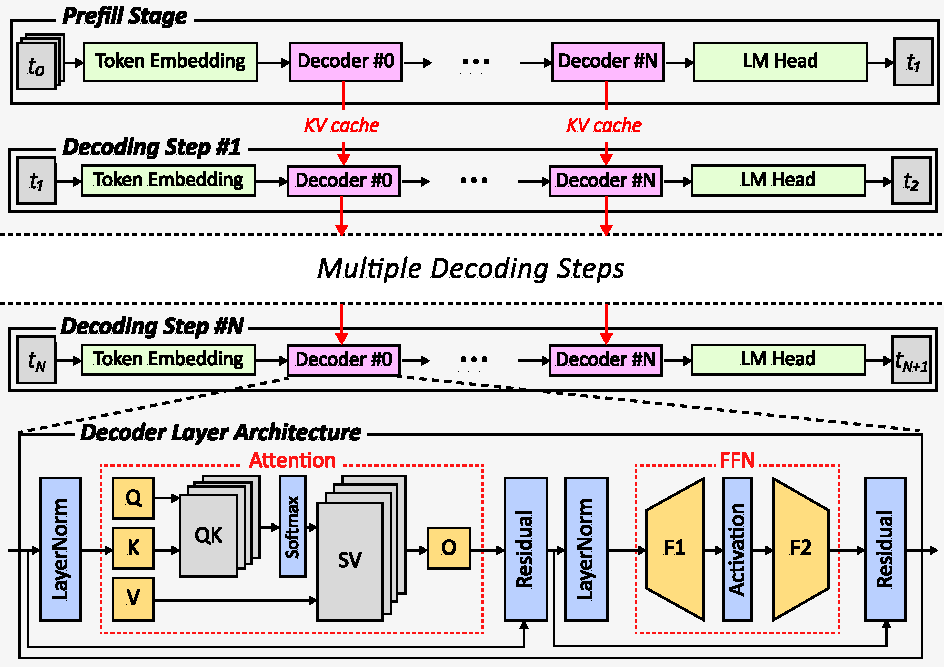
\includegraphics[width=\colimgwidth]{Figures/2_1_LLM_Architecture.pdf}
\caption{Architecture of autoregressive transformer based LLMs}
\label{fig_2_1}
\vspace{-1.5em}
\end{figure}


\subsection{Large Language Model Architecture}
\label{section_2_1}
Despite the exploration of alternative language model architectures~\cite{rnn-rwkv, mamba, llada}, the autoregressive transformer remains the dominant architecture for LLMs. Transformer fundamentally consists of two main layers: the multi-head attention and the feed-forward network. Figure~\ref{fig_2_1} illustrates the structure of a transformer layer, where the yellow modules denote weight–activation multiplications, the gray modules represent activation–activation multiplications, and the blue modules correspond to non-linear operations.

A defining characteristic of transformers in LLMs is their autoregressive nature. These models are trained to predict the next token conditioned on the preceding sequence. Consequently, text generation is performed through an autoregressive process, in which the entire accumulated sequence is repeatedly processed to produce each subsequent token. A naive implementation of this process incurs substantial redundant computation, as portions of the sequence remain unchanged across generation steps.

To mitigate this inefficiency, modern LLMs employ the Key-Value (KV) caching technique, which stores the key and value tensors generated by the attention layers and reuses them in subsequent iterations. The initial phase, where the model processes the input sequence and generates the first token, is referred to as the prefill stage. The subsequent token generation steps that leverage the KV cache constitute the decode stage. The prefill stage is dominated by large-scale matrix multiplications, resulting in high arithmetic intensity and substantial computational demand. In contrast, the decode stage exhibits significantly lower arithmetic intensity and is typically memory-bound on conventional parallel architectures.

% \subsection{Recent LLM Trends: Long Context Comprehension and Reasoning Capability}
% \label{section_2_2}

% The primary performance improvement in early LLMs was mainly achieved through increasing the size of the pretrained parameters. However, due to the enormous cost increases associated with scaling up model size, researchers have recently ceased simply increasing the number of parameters and are now attempting to enhance LLM performance through two new avenues.

% One direction is the expansion of context length. Early LLMs could only process a few thousand tokens, but recent LLMs now support context lengths in the millions. For example, one of the latest sLLMs, Qwen3-4B~\cite{Qwen3-4B} can process 200 times longer context compared to Llama-1-base, and this trend is expected to increase further.

% The second direction is the advancement of reasoning capability. Most recent LLMs can deal with complex tasks such as solving math problems and programming. This is because they undergo an additional reinforcement learning process after pretraining, utilizing high-quality reasoning problem datasets. From a workload perspective, the biggest difference between reasoning LLMs and non-reasoning LLMs is an increased decode stage ratio. Table~\ref{table_2_1} shows the difference in generated context length on the GPQA-Diamond benchmark~\cite{GPQA-Diamond} between two distinct models that share the same base model. As this table illustrates, even when sharing the same base model, reasoning LLMs generate sentences that are several times longer from the same input compared to non-reasoning LLMs. This phenomenon increases the proportion of the decode stage in modern LLMs.

% Therefore, consideration of long context processing capabilities and the extended decode stage is also essential for designing a modern LLM inference system.


\subsection{Speculative Decoding}
\label{section_2_3}

%%%%%%%%%%%%%%%%%%%%%%%%%%%%%%%%%%%%%%%%%%%%%%%%%%
\begin{figure}[t]
\centering
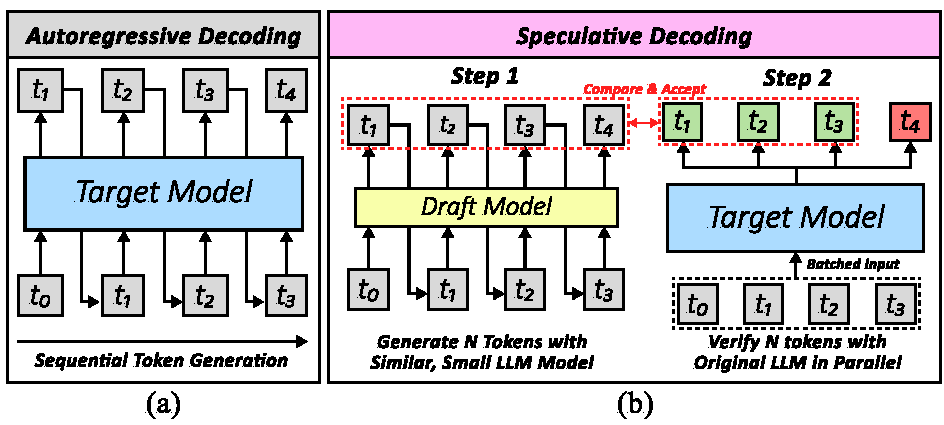
\includegraphics[width=\colimgwidth]{Figures/2_3_Speculative_Decoding.pdf}
\caption{(a) Autoregressive decoding. (b) speculative decoding.}
\label{fig_2_3}
\vspace{-1.5em}
\end{figure}
%%%%%%%%%%%%%%%%%%%%%%%%%%%%%%%%%%%%%%%%%%%%%%%%%%
% Based on this idea, a wide variety of parallel decoding techniques have recently emerged. Still, the method that uses two LLMs, a target model and a draft model, remains the most widely adopted~\cite{speculativedecoding}.

The core idea of speculative decoding is to transform the sequential token generation in the decode stage into parallel ones. Based on this idea, a wide variety of parallel decoding techniques have recently emerged. Still, the method that uses two LLMs, a target model and a draft model, remains the most widely adopted~\cite{speculativedecoding}.

Figure~\ref{fig_2_3} illustrates the difference between autoregressive decoding and speculative decoding. Here, the target model is the original LLM, and the draft model is a comparatively smaller LLM trained to generate tokens with a probability distribution similar to the target model. In this method, the draft model first generates a few tokens, and the target model subsequently verifies those tokens in parallel. To understand the performance gain afforded by speculative decoding through a simplified example, let us define the time required for the draft model to generate a single token as $t_{draft}$, and the time required for the target model to generate a single token as $t_{target}$. In a scenario involving $\gamma$ token generations via autoregressive decoding, the total time consumption would be $\gamma t_{target}$. However, consider the application of speculative decoding, where $\gamma$ tokens are first generated by the draft model and subsequently verified by the target model, assuming all $\gamma$ tokens are generated correctly. In this case, the target model performs batched inference by receiving $\gamma$ tokens from the draft model. Since $\gamma$ is generally not large, this batched inference operates as a memory-bound on commercial xPUs, and the time required for this is nearly equivalent to the time needed to generate a single token. Consequently, the total time taken in this scenario is approximated by $\gamma t_{draft}+t_{target}$. If $t_{draft}$ is sufficiently smaller than $t_{target}$, a substantial performance improvement is achieved.

% While the target model execution is still necessary, it processes the $\gamma$ tokens from the draft model in parallel. Given that the time required for an xPU with adequate computing resources to process $\gamma$ tokens in parallel is nearly equivalent to the time for generating a single token, the total time required in this specific scenario is approximated by $\gammat_{draft}+t_{target}$. If $t_{draft}$ is sufficiently smaller than $t_{target}$, a substantial performance improvement is achieved.

One problem arises in this process: the draft model does not always generate the correct tokens. If the draft model generates an incorrect token, the target model detects it during the verification process and only accepts tokens up to the one preceding the error as correctly generated. The criteria for accepting tokens generated by the draft model can vary depending on the scenario.

When utilizing greedy decoding, we can only accept the output if the draft model produces the identical token. Under this condition, the target model's output remains perfectly preserved by speculative decoding. In contrast, recent LLMs often employ sampling techniques that introduce a degree of randomness during the new token generation process.
In such a scenario, to maintain appropriate randomness, a probability-based sampling method~\cite{speculativesampling}, often expressed by the equation below, is frequently employed.

\begin{equation}
n \leftarrow \min\left(\left\{i-1 \middle| 1 \leq i \leq \gamma, r_i > \frac{p_i(x)}{q_i(x)}\right\} \cup \{\gamma\}\right)
\end{equation}
\vspace{0.05in}

Here, $n$ is the number of accepted tokens, $\gamma$ is the draft length, $i$ is the index, $r_i$ is a random probability between 0 and 1, $p_i(x)$ is the probability of the $i$-th token obtained from the target model's logits, and $q_i(x)$ is the probability of the $i$-th token obtained from the draft model's logits. This approach is known as rejection sampling, and with this method, the entire speculative decoding system is mathematically guaranteed to generate tokens that are probabilistically identical to those of the target model.

The ratio in which the draft model correctly predicts how many tokens on average is called the acceptance rate. Since a low acceptance rate for the draft model can lead to a performance degradation in speculative decoding, it is crucial to develop a draft model that is both fast and has a sufficiently high acceptance rate.

% By using this approach, it is mathematically guaranteed that using speculative decoding results in the generation of sentences with the same level of quality as the target model.
